\documentclass[svgnames,11pt]{beamer}
\input{/home/tof/Documents/Cozy/latex-include/preambule_commun.tex}
\input{/home/tof/Documents/Cozy/latex-include/preambule_beamer.tex}
%\usepackage{pgfpages} \setbeameroption{show notes on second screen=left}
\author[]{Christophe Viroulaud}
\title{Rentrée 2J}
\date{\framebox{\textbf{}}}
%\logo{}
\institute{Seconde - SNT}

\begin{document}
\begin{frame}
    \titlepage
\end{frame}
\begin{frame}
    \frametitle{Vérification de la liste}

    \begin{aretenir}[Remarque]
        Toute de demande de changement de régime devra être adressée par courrier à l'intendance avant le 10 septembre.
    \end{aretenir}

\end{frame}
\begin{frame}
    \frametitle{Emploi du temps}

    \begin{center}
        \centering
        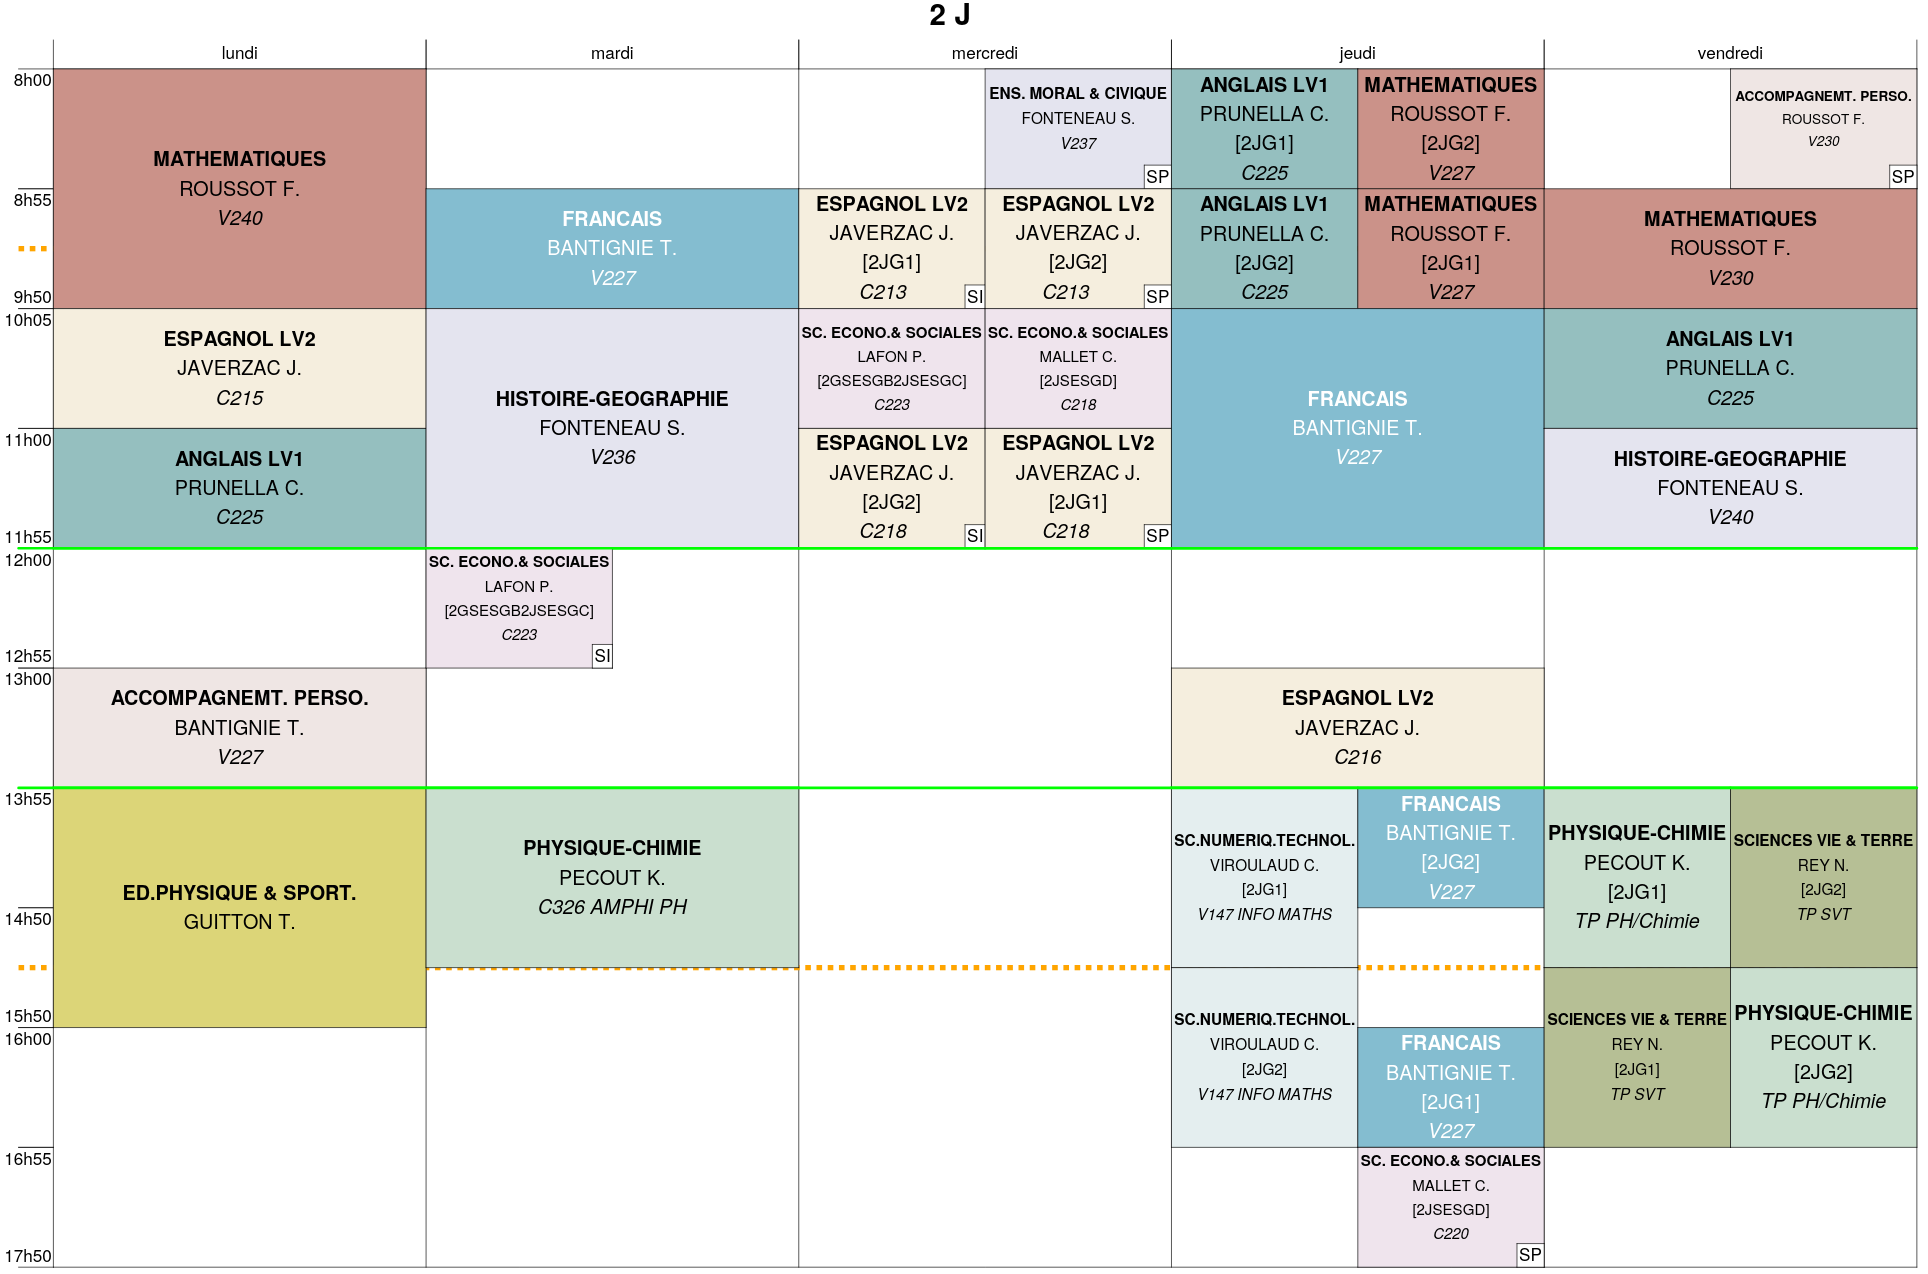
\includegraphics[width=10cm]{2j2021.png}
    \end{center}
\end{frame}
\begin{frame}
    \frametitle{}


    \begin{aretenir}[remarque]
        Nous commençons en semaine impaire. Le calendrier est disponible sur Pronote.
    \end{aretenir}

\end{frame}
\begin{frame}
    \frametitle{Protocole sanitaire}

    \begin{itemize}
        \item masque
        \item gel hydroalcoolique
        \item distanciation
        \item pas de stationnement dans les couloirs
        \item sens de circulation
    \end{itemize}

\end{frame}
\begin{frame}
    \frametitle{Visite du lycée}

    \begin{center}
        \centering
        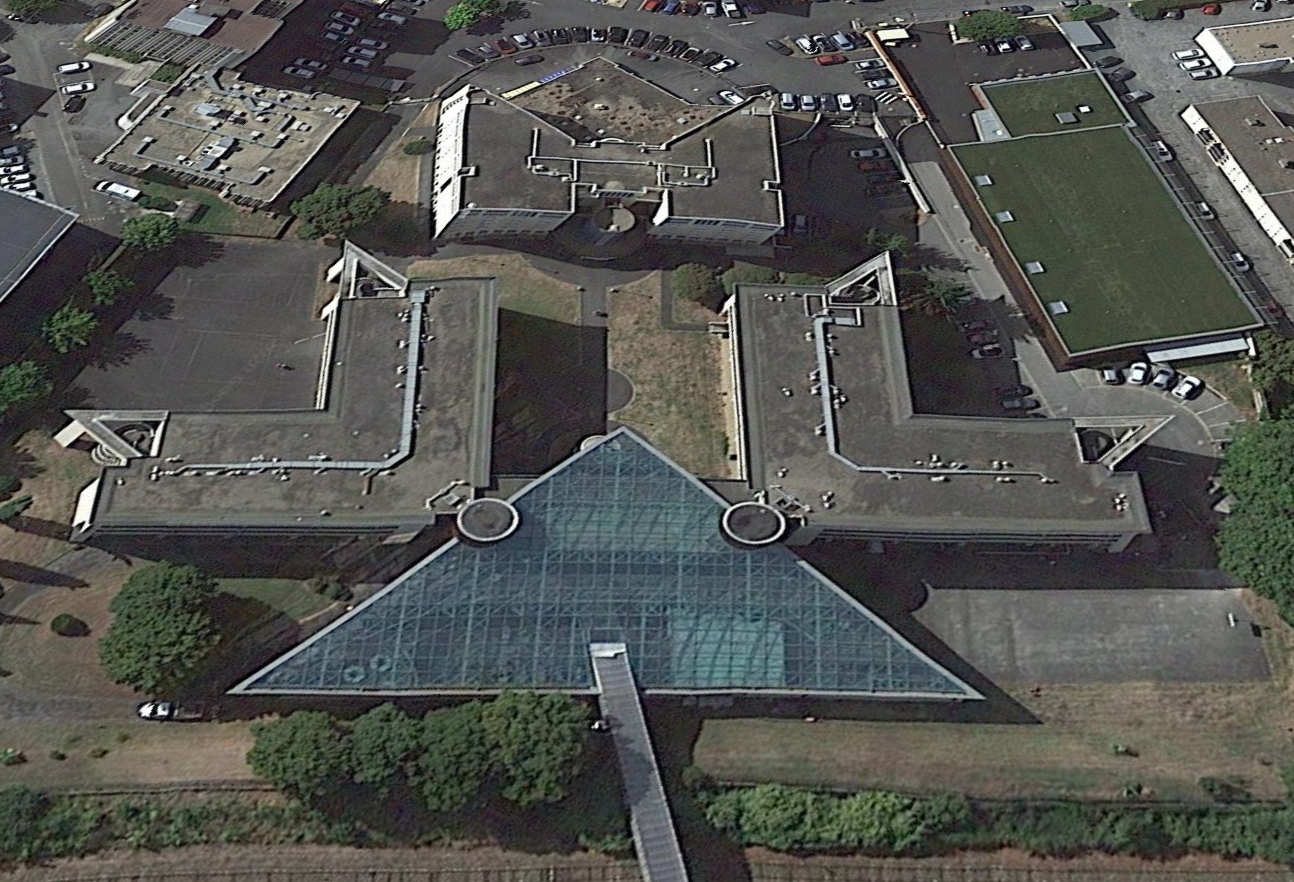
\includegraphics[width=10cm]{jay.png}
    \end{center}

\end{frame}
\begin{frame}
    \frametitle{Codes}

    \begin{itemize}
        \item Pronote
        \item Educonnect
    \end{itemize}
    \begin{aretenir}[Remarque]
        Pour accéder à ces plateformes, le plus simple est de se rendre sur le site \url{https://lyceejaydebeaufort.fr/}
    \end{aretenir}
\end{frame}
\begin{frame}
    \frametitle{Administratif}

    \begin{itemize}
        \item Autorisation à la vaccination
        \item distribution des manuels: vendredi 3 septembre à 15h30
        \item rencontre équipe de direction: mardi 7 septembre de 14h à 14h30
        \item Tests de positionnement
    \end{itemize}

\end{frame}
\begin{frame}
    \frametitle{Repas}

    \begin{itemize}
        \item \textbf{self en rénovation:} restauration dans les structures à l'entrée du lycée.
        \item Pour les DP et internes: cartes remises prochainement par la vie scolaire.
        \item En cas de cours entre 12h et 14h les internes peuvent manger au self (ticket à l'intendance).
    \end{itemize}

\end{frame}
\begin{frame}
    \frametitle{Règlement intérieur}

    \begin{itemize}
        \item<1-> Obligations scolaires
              \begin{itemize}
                  \item travail et résultats
                  \item assiduité et ponctualité
              \end{itemize}
        \item <2-> Régime des entrées - sorties
        \item <3-> Tenue et comportement
    \end{itemize}

\end{frame}
\begin{frame}
    \frametitle{Début des cours}

    \begin{aretenir}[]\centering
        {\Large     Les cours commencent vendredi 3 septembre à 8h.
        }    \end{aretenir}

\end{frame}
\end{document}